\section{Simulation}
To simulate the Touschek Effect, we do something similar to what Khan has done in [4], and adopt it to work with particle tracking.\\
Here is the plan:
\begin{enumerate}
\item Use linear optics to simulate the motion of the electrons around the storage ring.
\item Pick out 2 particles/particle coordinates at random. (one of each electron in the bunch)
\item Pick out 2 scattering angles at random $\Theta \in \left[\epsilon,\pi/2\right], \Phi \in \left[0,\pi\right]$, with $\epsilon > 0$ but small..
\item Check if particles are outside momenta acceptance (see scattering at an angle on how to do it), if no. Go back to 2, if yes go on.
% \item Get the particle densities at the 2 particles.
\item Do some math written down below.
\end{enumerate}
The cross section in the center of momentum frame is given by:
\begin{equation} \sigma = \frac{r_e ^2}{4} \left(1 - \frac{v^2}{c^2}\right) \left[ (X+1)^2 \left(\frac 4 {\sin^4 \Theta} - \frac 3 {\sin^2 \Theta}\right) + 1 + \frac 4 {\sin^2 \Theta}\right] \end{equation}
with
\begin{equation} X = \left(\frac c v\right)^2 = \beta^{-2} = \frac{\gamma^2}{\gamma^2 - 1} \end{equation}
see the theory section for more details.\\
For each event we compute:
\begin{equation} \Delta u = 2 v \sin \Theta \sigma \rho_1 \rho_2, \ v = v(p_1 - p_2) \end{equation}
or something similar. Where $\sigma \rightarrow \sigma \cdot \gamma$ to transform from the center of momenta system into the bunch system and $v$ is taken in the bunch system. This is different from what Khan did in [4].\\
Having done all theses computations along one turn, we compute:
\begin{equation} \alpha = \frac{\Delta V} n \frac {1}{\gamma C} \sum\limits_{\delta p > \Delta p} \Delta u. \end{equation}
The sum is taken over all events around the storage ring, where we passed the momentum acceptance. Here C is the circumference of the storage ring. $\gamma$ is the one to go from the bunch to the laboratory frame. Where $\Delta V$ is our total volume, we are picking events out,  given by:
\begin{equation} \Delta V = (2 a)^9 \sum\limits_C \sigma_x \sigma_y \sigma_z (\sigma_{x'} \sigma_{y'} \sigma_{z'})^2 l \cdot \pi^2 / 2. \end{equation}
Where the sum is evaluated along the circumference of the storage ring, and l being the length of one step. Assuming we are scattering each electron in the bunch on each time step, we will have:
\begin{equation} N_{events} = N_{sim} \cdot N_{timestep}. \end{equation}
\subsection{Why Epsilon?}
I wrote before, that we are  picking $\Theta \in \left[\epsilon,\pi/2\right]$ with $\epsilon > 0$ but small. This has the reason that the cross section $\sigma$ diverges as $\Theta \rightarrow 0$, so we need to stop at some angle $\Theta_{min}$. The physical reason behind this divergence is that the Coulomb force doesn't have a cutoff at a certain length, but reaches to infinity. This problem doesn't only arise with our relativistic cross section, but also in the classical one.
\subsubsection{Estimate of Epsilon}
Using a similar Approach as Dawson does in [9] to estimate the collisional effect, we suppose, that the momentum change is given by:
\begin{equation} \Delta P = F(\rho) \cdot \frac{2 \rho} v \end{equation}
here F is the force function, $\rho$ the impact parameter and v the speed of the particle. We can suppose that the impact parameter is in the size of the Debye length, and that the force works tangential to the momenta of the particle. This leads us to a scattering angle of:
\begin{equation} \tan \Theta = \frac{\Delta P}{P}. \end{equation}
So we get the final expression:
\begin{equation} \tan \Theta = \frac{q_e ^2}{2 \pi \epsilon_0 m_e} \cdot \frac{\rho}{v^2}. \end{equation}
This estimate is based on, that we are allowed to use non-relativistic mechanics, which is wrong.\\
Using this estimate we find with $\rho = \lambda_D$ and $v = \sigma_{x'} \cdot c$, that scatterings under an angle of $10^{-6}$ won't happen.
\subsection{Different simulation approaches}

\subsubsection{Analytical Approach}
Using a fully analytic approach we pick out the particles at random out of an uniform distribution. So we follow exactly what S.Khan has done in [10].
\begin{equation} - a \cdot \sigma_x < x < a \cdot \sigma_x, \ \ -a \cdot \sigma_{x'} - x \cdot \alpha_x / \beta_x < x' <a \cdot \sigma_{c'} - x \cdot \alpha_x / \beta_x \end{equation} 
and the same for y and z. Here a designs the sigma width we are using, and $\alpha_x$ and $\beta_x$ are the Twiss Parameters. We are also using the full volume element given above:
\begin{equation} \Delta V = (2 a)^9 \sum\limits_C \sigma_x \sigma_y \sigma_z (\sigma_{x'} \sigma_{y'} \sigma_{z'})^2 l \cdot \pi^2 / 2. \end{equation}
We are determining the density of finding a particle at $\vec R = (x,y,z)$ with momenta $\vec P / P_0 = (x', y', z')$ using:
\begin{equation} \rho = \rho_x \cdot \rho_y \cdot \rho_z \end{equation}
with
\begin{equation} \rho_x = \frac 1 {2 \pi \epsilon_x} e^{\left(- \frac 1 {2 \epsilon_x}(\gamma_x x^2 + 2 \alpha_x x x' + \beta_x x'^2)\right)} \end{equation}
and similar expressions for $\rho_y$ and $\rho_z$. For $\rho_z$ the term in $2 \alpha_z z z'$ is omitted. Here $\alpha_x, \beta_x$ and $\gamma_x$ are the Twiss parameters and $\epsilon_x$ is the emittance.

\subsubsection{Semianalytical Approach}
If we are chosen one particle out of the bunch as interaction partner. We are already weighting the choice, because our bunch is gaussian distributed. So we will have to make some modifications, we have a smaller random volume, given by:
\begin{equation} \Delta \hat V = (2 a)^3 \sum\limits_C \sigma_{x'} \sigma_{y'} \sigma_{z'} l \cdot \pi^2 / 2. \end{equation}
Because only the momentum of the second particle is random. And also:
\begin{equation} \Delta \hat u = 2 v \sin \Theta \sigma \rho_2, \ v = v(p_1 - p_2) \end{equation}
because the first particle already is weighted in.

\subsubsection{2 Particles Approach}
I am still not sure how to do it with the second particle, and if it possible. I have tried the same approach, leaving only the scattering angles as random variables. This would lead to the change in formulas to:
\begin{equation} \Delta \tilde V = \sum\limits_C l \cdot \pi^2 / 2 \end{equation}
and
\begin{equation} \Delta \tilde u = 2 v \sin \Theta \sigma, \ v = v(p_1 - p_2). \end{equation}
Which requires just using 2 randomly chosen particles out of the bunch, where from the second one we only use the momenta coordinate.\\
This doesn't give the same result as the 2 approaches before (they do in good approximation), this is probably because the probably for the momenta is taken at a different place then where the interaction takes place.\\
It might be worth a try only using electrons inside the Debye Sphere as possible candidates for the random collision.

\pagebreak

\section{Validation}
First tries with the simulation of Aurora showed that all the above approaches lead to good results for $\alpha$. Although they don't fall completely together with experimental or theoretical results. However this can be expected because we are not taking into account such as beam polarizations or synchrotron radiation.\\
\begin{figure}[here]
 \centering
 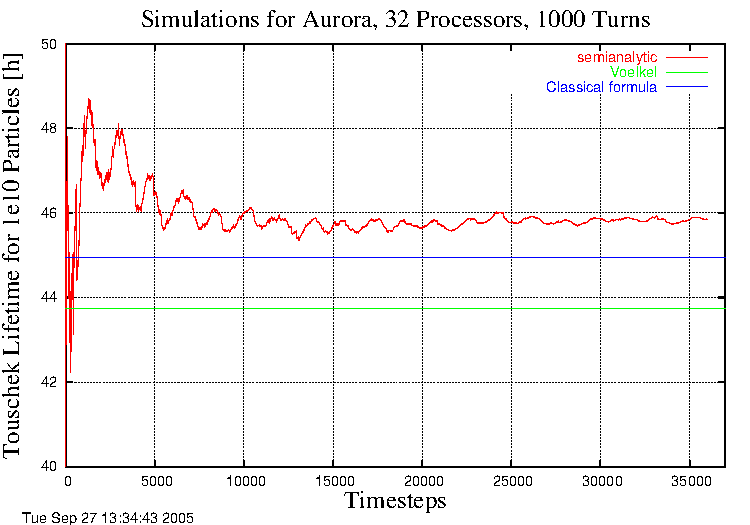
\includegraphics[width=0.80\textwidth]{aurlong.pdf}
 \caption{Aurora Simulation}
\end{figure}
The not falling together with the result from the formulas can be also expected, since these formulas use one fixed beam geometry, and in our simulation the beam geometry is changing.\\
The newer results shows, that for different $\gamma$ the deviation of the V\"olkel and the ZAP calculations are bigger, then the ones from our model.\\
In the following we will compare our different ways of computing the lifetime. Since also these results differ from each other.

\subsection{Semianalytic vs. Analytic}
\begin{figure}[here]
 \centering
 \includegraphics[width=0.80\textwidth]{sls-conv-1.pdf}
 \caption{Longterm Behavior}
\end{figure}
This figure shows that the analytic and semi-analytic approaches of computing the scattering rates stay very close to each other. It also shows that the semianalytic approach has a much better convergence, then the full analytic one. This is probably caused by the particles being picked out at places of statistical importance. It might be worth a try switching from an uniform random number generator to a gaussian one, dropping the densities, and test if we have better convergence with still the same result.\\
For other settings (Aurora simulation), we had full convergence between analytic and semianalytic cases. The non-convergence here might be due to not long enough computation times.
\subsection{2 Particle Approach}
\begin{figure}[here]
 \centering
 \includegraphics[width=0.80\textwidth]{sls-conv-2.pdf}
 \caption{Longterm Behavior}
\end{figure}
The difference between the 2 particle version and the analytic ones, is that the second momenta is taken in the analytic ones where the interaction takes place, for the 2 particle one, we have the probability of finding the momenta somewhere in the beam. This means that it might be interesting to test what happens if we pick particles that are close to each other.

\subsection{Known Drawbacks}
\begin{itemize}
\item We are only simulating Touschek loss, other effects as scattering from residual gas influence the lifetime.
\item If a part of a particle is lost, it is not taken out of the beam.
\item We have no synchrotron radiation.
\item We are only using linear optics.
\end{itemize}

\subsection{Units}
In the simulation the following units are being used. The spatial coordinates are given in meter. The momentum coordinates are given as relative coordinates to a reference momentum. So they are unit less.

